\section{Let3d Class Reference}
\label{classLet3d}\index{Let3d@{Let3d}}
{\tt \#include $<$let3d.hpp$>$}

Inheritance diagram for Let3d::\begin{figure}[H]
\begin{center}
\leavevmode
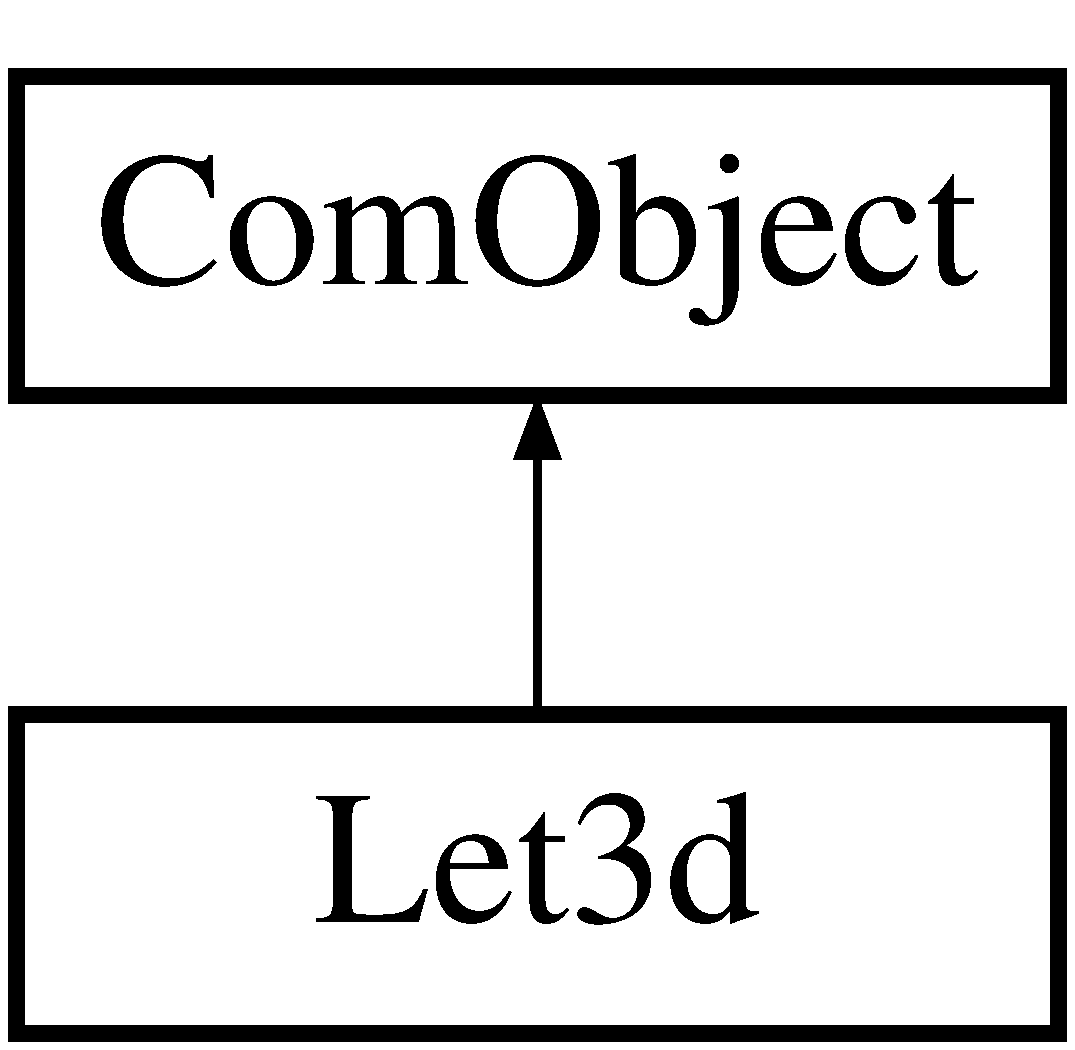
\includegraphics[height=2cm]{classLet3d}
\end{center}
\end{figure}


\subsection{Detailed Description}




Definition at line 34 of file let3d.hpp.\subsection*{Public Member Functions}
\begin{CompactItemize}
\item 
{\bf Let3d} (const string \&p)
\item 
{\bf $\sim$Let3d} ()
\item 
Dbl\-Num\-Mat $\ast$\& {\bf src\-Pos} ()
\item 
Dbl\-Num\-Mat $\ast$\& {\bf trg\-Pos} ()
\item 
Point3 \& {\bf center} ()
\item 
int \& {\bf root\-Level} ()
\item 
double {\bf radius} ()
\item 
int \& {\bf pts\-Max} ()
\item 
int \& {\bf max\-Level} ()
\item 
int {\bf setup} (map$<$ string, string $>$ \&opts)
\item 
int {\bf print} ()
\item 
vector$<$ {\bf Node} $>$ \& {\bf node\-Vec} ()
\item 
int {\bf src\-Node\-Cnt} ()
\item 
int {\bf src\-Exa\-Cnt} ()
\item 
int {\bf trg\-Node\-Cnt} ()
\item 
int {\bf trg\-Exa\-Cnt} ()
\item 
int {\bf src\-Data} ()
\item 
int {\bf trg\-Data} ()
\item 
int {\bf calgnext} (int g\-Node\-Idx)
\item 
int {\bf dwn\-Order\-Collect} (vector$<$ int $>$ \&)
\item 
int {\bf upw\-Order\-Collect} (vector$<$ int $>$ \&)
\item 
{\bf Node} \& {\bf node} (int g\-Node\-Idx)
\item 
bool {\bf root} (int g\-Node\-Idx)
\item 
bool {\bf terminal} (int g\-Node\-Idx)
\item 
int {\bf parent} (int g\-Node\-Idx)
\item 
int {\bf child} (int g\-Node\-Idx, const Index3 \&idx)
\item 
Index3 {\bf path2Node} (int g\-Node\-Idx)
\item 
int {\bf depth} (int g\-Node\-Idx)
\item 
int {\bf tag} (int g\-Node\-Idx)
\item 
Point3 {\bf center} (int g\-Node\-Idx)
\item 
double {\bf radius} (int g\-Node\-Idx)
\item 
int {\bf findgnt} (int depth, const Index3 \&path2Node)
\item 
bool {\bf adjacent} (int, int)
\item 
int {\bf dim} () const 
\end{CompactItemize}
\subsection*{Protected Attributes}
\begin{CompactItemize}
\item 
Dbl\-Num\-Mat $\ast$ {\bf \_\-src\-Pos}
\item 
Dbl\-Num\-Mat $\ast$ {\bf \_\-trg\-Pos}
\item 
Point3 {\bf \_\-center}
\item 
int {\bf \_\-root\-Level}
\item 
int {\bf \_\-pts\-Max}
\item 
int {\bf \_\-max\-Level}
\item 
vector$<$ {\bf Node} $>$ {\bf \_\-node\-Vec}
\item 
int {\bf \_\-level}
\item 
int {\bf \_\-src\-Node\-Cnt}
\item 
int {\bf \_\-src\-Exa\-Cnt}
\item 
int {\bf \_\-trg\-Node\-Cnt}
\item 
int {\bf \_\-trg\-Exa\-Cnt}
\end{CompactItemize}
\subsection*{Classes}
\begin{CompactItemize}
\item 
class {\bf Node}
\end{CompactItemize}


\subsection{Constructor \& Destructor Documentation}
\index{Let3d@{Let3d}!Let3d@{Let3d}}
\index{Let3d@{Let3d}!Let3d@{Let3d}}
\subsubsection{\setlength{\rightskip}{0pt plus 5cm}Let3d::Let3d (const string \& {\em p})}\label{classLet3d_f8d536a83eec83f76c37ef8ab65ca50a_f8d536a83eec83f76c37ef8ab65ca50a}




Definition at line 30 of file let3d.cpp.

\footnotesize\begin{verbatim}30                            :
31   ComObject(p), _srcPos(NULL), _trgPos(NULL), _center(0.0), _rootLevel(0),
32   _ptsMax(150), _maxLevel(10)
33 {
34 }

\end{verbatim}\normalsize 


\index{Let3d@{Let3d}!~Let3d@{$\sim$Let3d}}
\index{~Let3d@{$\sim$Let3d}!Let3d@{Let3d}}
\subsubsection{\setlength{\rightskip}{0pt plus 5cm}Let3d::$\sim$Let3d ()}\label{classLet3d_b2dea69683e4c627d67f9de0f72909c1_b2dea69683e4c627d67f9de0f72909c1}




Definition at line 36 of file let3d.cpp.

\footnotesize\begin{verbatim}37 {
38 }
\end{verbatim}\normalsize 




\subsection{Member Function Documentation}
\index{Let3d@{Let3d}!adjacent@{adjacent}}
\index{adjacent@{adjacent}!Let3d@{Let3d}}
\subsubsection{\setlength{\rightskip}{0pt plus 5cm}bool Let3d::adjacent (int, int)}\label{classLet3d_a20d0c310a6e8d02f6295983c199c06f_a20d0c310a6e8d02f6295983c199c06f}




Definition at line 372 of file let3d.cpp.

References depth(), path2Node(), and radius().

Referenced by calgnext().

\footnotesize\begin{verbatim}373 {
374   int md = max(depth(me),depth(yo));
375   Index3 one(1);
376   Index3 mecenter(  (2*path2Node(me)+one) * pow2(md - depth(me))  );
377   Index3 yocenter(  (2*path2Node(yo)+one) * pow2(md - depth(yo))  );
378   int meradius = pow2(md - depth(me));
379   int yoradius = pow2(md - depth(yo));
380   Index3 dif( abs(mecenter-yocenter) );
381   int radius  = meradius + yoradius;
382   return
383          ( dif <= Index3(radius) ) && //not too far
384          ( dif.linfty() == radius ); //at least one edge touch
385 }
\end{verbatim}\normalsize 


\index{Let3d@{Let3d}!calgnext@{calgnext}}
\index{calgnext@{calgnext}!Let3d@{Let3d}}
\subsubsection{\setlength{\rightskip}{0pt plus 5cm}int Let3d::calgnext (int {\em g\-Node\-Idx})}\label{classLet3d_a57baa80b52cce7a3e0430c3bd3e6107_a57baa80b52cce7a3e0430c3bd3e6107}


build U,V,W,X lists 

Definition at line 234 of file let3d.cpp.

References adjacent(), depth(), findgnt(), node\-Vec(), parent(), path2Node(), root(), and terminal().

\footnotesize\begin{verbatim}235 {
236   vector<Node>&  nodeVec = this->nodeVec();
237   
238   set<int> Uset, Vset, Wset, Xset;
239   int curGNodeIdx = gNodeIdx;
240   if(root(curGNodeIdx)==false) {
241          int parGNodeIdx = parent(curGNodeIdx);
242          
243          Index3 minIdx(0);
244          Index3 maxIdx(pow2(depth(curGNodeIdx)));
245 
246          for(int i=-2; i<4; i++) {
247                 for(int j=-2; j<4; j++) {
248                   for(int k=-2; k<4; k++) {
249                          Index3 tryPath( 2*path2Node(parGNodeIdx) + Index3(i,j,k) );
250                          if(tryPath >= minIdx && tryPath <  maxIdx && tryPath != path2Node(curGNodeIdx)) {      
251                                 int resGNodeIdx = findgnt(depth(curGNodeIdx), tryPath);
252                                 bool adj = adjacent(resGNodeIdx, curGNodeIdx);
253                                 if( depth(resGNodeIdx) < depth(curGNodeIdx) ) {
254                                   if(adj){
255                                          if(terminal(curGNodeIdx)){
256                                                 Uset.insert(resGNodeIdx);
257                                          }
258                                          else { ; }
259                                   }
260                                   else {
261                                          Xset.insert(resGNodeIdx);
262                                   }
263                                 }
264                                 if( depth(resGNodeIdx)==depth(curGNodeIdx) ) {
265                                   if(!adj) {
266                                          Index3 bb(path2Node(resGNodeIdx)-path2Node(curGNodeIdx));
267                                          assert( bb.linfty()<=3 );
268                                          Vset.insert(resGNodeIdx);
269                                   }
270                                   else {
271                                          if(terminal(curGNodeIdx)) {
272                                                 queue<int> rest;
273                                                 rest.push(resGNodeIdx);
274                                                 while(rest.empty()==false) {
275                                                   int fntGNodeIdx = rest.front(); rest.pop();                                    //int fntgNodeIdx = fntgnt.gNodeIdx();
276                                                   if(adjacent(fntGNodeIdx, curGNodeIdx)==false) {
277                                                          Wset.insert( fntGNodeIdx );
278                                                   }
279                                                   else {
280                                                          if(terminal(fntGNodeIdx)) {
281                                                                 Uset.insert(fntGNodeIdx);
282                                                          }
283                                                          else { 
284                                                                 for(int a=0; a<2; a++) {
285                                                                   for(int b=0; b<2; b++) {
286                                                                          for(int c=0; c<2; c++) {
287                                                                                 rest.push( child(fntGNodeIdx, Index3(a,b,c)) );
288                                                                          }
289                                                                   }
290                                                                 }
291                                                          }
292                                                   }
293                                                 }
294                                          }
295                                   }
296                                 }
297                          }
298                   }
299                 }
300          }
301   }
302   if(terminal(curGNodeIdx))
303          Uset.insert(curGNodeIdx);
304   
305   for(set<int>::iterator si=Uset.begin(); si!=Uset.end(); si++)
306          if(nodeVec[*si].tag() & LET_SRCNODE)           nodeVec[gNodeIdx].Unodes().push_back(*si);
307   for(set<int>::iterator si=Vset.begin(); si!=Vset.end(); si++)
308          if(nodeVec[*si].tag() & LET_SRCNODE)           nodeVec[gNodeIdx].Vnodes().push_back(*si);
309   for(set<int>::iterator si=Wset.begin(); si!=Wset.end(); si++)
310          if(nodeVec[*si].tag() & LET_SRCNODE)           nodeVec[gNodeIdx].Wnodes().push_back(*si);
311   for(set<int>::iterator si=Xset.begin(); si!=Xset.end(); si++)
312          if(nodeVec[*si].tag() & LET_SRCNODE)           nodeVec[gNodeIdx].Xnodes().push_back(*si);
313   
314   return (0);
315 }
\end{verbatim}\normalsize 


\index{Let3d@{Let3d}!center@{center}}
\index{center@{center}!Let3d@{Let3d}}
\subsubsection{\setlength{\rightskip}{0pt plus 5cm}Point3 Let3d::center (int {\em g\-Node\-Idx})}\label{classLet3d_dff5f922c11176af18f4bfa95c138a20_dff5f922c11176af18f4bfa95c138a20}




Definition at line 342 of file let3d.cpp.

References center(), depth(), dim(), path2Node(), and radius().

\footnotesize\begin{verbatim}343 {
344   Point3 ll( center() - Point3(radius()) );
345   int tmp = pow2(depth(gNodeIdx));
346   Index3 pathLcl(path2Node(gNodeIdx));
347   Point3 res;
348   for(int d=0; d<dim(); d++) {
349          res(d) = ll(d) + (2*radius()) * (pathLcl(d)+0.5) / double(tmp);
350   }
351   return res;
352 }
\end{verbatim}\normalsize 


\index{Let3d@{Let3d}!center@{center}}
\index{center@{center}!Let3d@{Let3d}}
\subsubsection{\setlength{\rightskip}{0pt plus 5cm}Point3\& Let3d::center ()\hspace{0.3cm}{\tt  [inline]}}\label{classLet3d_5c0517b22b09f08712cbfd01aa1f29d7_5c0517b22b09f08712cbfd01aa1f29d7}




Definition at line 122 of file let3d.hpp.

References \_\-center.

Referenced by center(), src\-Data(), and trg\-Data().

\footnotesize\begin{verbatim}122 { return _center; }
\end{verbatim}\normalsize 


\index{Let3d@{Let3d}!child@{child}}
\index{child@{child}!Let3d@{Let3d}}
\subsubsection{\setlength{\rightskip}{0pt plus 5cm}int Let3d::child (int {\em g\-Node\-Idx}, const Index3 \& {\em idx})}\label{classLet3d_127278ccf71ca1d7a807d7531be1ad40_127278ccf71ca1d7a807d7531be1ad40}




Definition at line 337 of file let3d.cpp.

References Let3d::Node::child(), and node().

Referenced by findgnt().

\footnotesize\begin{verbatim}338 {
339   assert(idx>=Index3(0) && idx<Index3(2));
340   return node(gNodeIdx).child() + (idx(0)*4+idx(1)*2+idx(2));
341 }
\end{verbatim}\normalsize 


\index{Let3d@{Let3d}!depth@{depth}}
\index{depth@{depth}!Let3d@{Let3d}}
\subsubsection{\setlength{\rightskip}{0pt plus 5cm}int Let3d::depth (int {\em g\-Node\-Idx})\hspace{0.3cm}{\tt  [inline]}}\label{classLet3d_365114de1453e803d05b02702d1e0bc2_365114de1453e803d05b02702d1e0bc2}




Definition at line 156 of file let3d.hpp.

References Let3d::Node::depth(), and node().

Referenced by adjacent(), calgnext(), center(), findgnt(), and radius().

\footnotesize\begin{verbatim}156 { return node(gNodeIdx).depth(); }
\end{verbatim}\normalsize 


\index{Let3d@{Let3d}!dim@{dim}}
\index{dim@{dim}!Let3d@{Let3d}}
\subsubsection{\setlength{\rightskip}{0pt plus 5cm}int Let3d::dim () const\hspace{0.3cm}{\tt  [inline]}}\label{classLet3d_3b54adb16617f4dccdd399f842f3f6bf_3b54adb16617f4dccdd399f842f3f6bf}




Definition at line 165 of file let3d.hpp.

Referenced by center(), src\-Data(), and trg\-Data().

\footnotesize\begin{verbatim}165 { return 3; }  
\end{verbatim}\normalsize 


\index{Let3d@{Let3d}!dwnOrderCollect@{dwnOrderCollect}}
\index{dwnOrderCollect@{dwnOrderCollect}!Let3d@{Let3d}}
\subsubsection{\setlength{\rightskip}{0pt plus 5cm}int Let3d::dwn\-Order\-Collect (vector$<$ int $>$ \&)}\label{classLet3d_1917ece529ea97f12e74e56e42b6d15a_1917ece529ea97f12e74e56e42b6d15a}


top down ordering of the nodes 

Definition at line 317 of file let3d.cpp.

References \_\-\_\-FUNCT\_\-\_\-, and node\-Vec().

\footnotesize\begin{verbatim}318 {
319   orderBoxesVec.clear();
320   for(int i=0; i < nodeVec().size(); i++)
321          orderBoxesVec.push_back(i);
322   iA(orderBoxesVec.size()==nodeVec().size());
323   return 0;
324 }
\end{verbatim}\normalsize 


\index{Let3d@{Let3d}!findgnt@{findgnt}}
\index{findgnt@{findgnt}!Let3d@{Let3d}}
\subsubsection{\setlength{\rightskip}{0pt plus 5cm}int Let3d::findgnt (int {\em depth}, const Index3 \& {\em path2Node})}\label{classLet3d_dadf07c3ca29b244d01e8570e2846a2c_dadf07c3ca29b244d01e8570e2846a2c}




Definition at line 358 of file let3d.cpp.

References child(), depth(), and terminal().

Referenced by calgnext().

\footnotesize\begin{verbatim}359 {
360   int cur = 0;  //cerr<<"GOOD "<<path(cur)<<"     ";
361   Index3 leftpath(wntpath);
362   while(depth(cur)<wntdepth && terminal(cur)==false) {
363          int dif = wntdepth-depth(cur);
364          int tmp = pow2(dif-1);
365          Index3 choice( leftpath/tmp );
366          leftpath -= choice*tmp;
367          cur = child(cur, choice);       //cur = child(cur, IdxIter(0,2,true,choice) );  //cerr<<path(cur)<<"["<<choice<<" "<<tmp<<"]"<<"     ";
368   }  //cerr<<endl;
369   return cur;
370 }
\end{verbatim}\normalsize 


\index{Let3d@{Let3d}!maxLevel@{maxLevel}}
\index{maxLevel@{maxLevel}!Let3d@{Let3d}}
\subsubsection{\setlength{\rightskip}{0pt plus 5cm}int\& Let3d::max\-Level ()\hspace{0.3cm}{\tt  [inline]}}\label{classLet3d_fdc3ca03e415e2d7b0b1f708d3ab94bb_fdc3ca03e415e2d7b0b1f708d3ab94bb}




Definition at line 126 of file let3d.hpp.

References \_\-max\-Level.

\footnotesize\begin{verbatim}126 { return _maxLevel; }
\end{verbatim}\normalsize 


\index{Let3d@{Let3d}!node@{node}}
\index{node@{node}!Let3d@{Let3d}}
\subsubsection{\setlength{\rightskip}{0pt plus 5cm}{\bf Node}\& Let3d::node (int {\em g\-Node\-Idx})\hspace{0.3cm}{\tt  [inline]}}\label{classLet3d_f259ccf218dbf0a04530841785f1a8b0_f259ccf218dbf0a04530841785f1a8b0}


node access 

Definition at line 148 of file let3d.hpp.

References \_\-node\-Vec.

Referenced by child(), depth(), FMM3d::evaluate(), parent(), path2Node(), print(), root(), FMM3d::src\-Data(), FMM3d::src\-Exa\-Den(), FMM3d::src\-Exa\-Nor(), FMM3d::src\-Exa\-Pos(), FMM3d::src\-Upw\-Chk\-Val(), FMM3d::src\-Upw\-Equ\-Den(), tag(), terminal(), FMM3d::trg\-Data(), FMM3d::trg\-Dwn\-Chk\-Val(), FMM3d::trg\-Dwn\-Equ\-Den(), FMM3d::trg\-Exa\-Pos(), and FMM3d::trg\-Exa\-Val().

\footnotesize\begin{verbatim}148 { return _nodeVec[gNodeIdx]; }
\end{verbatim}\normalsize 


\index{Let3d@{Let3d}!nodeVec@{nodeVec}}
\index{nodeVec@{nodeVec}!Let3d@{Let3d}}
\subsubsection{\setlength{\rightskip}{0pt plus 5cm}vector$<${\bf Node}$>$\& Let3d::node\-Vec ()\hspace{0.3cm}{\tt  [inline]}}\label{classLet3d_44c0c8da466878274feb4ce060c10b9b_44c0c8da466878274feb4ce060c10b9b}




Definition at line 131 of file let3d.hpp.

References \_\-node\-Vec.

Referenced by calgnext(), dwn\-Order\-Collect(), src\-Data(), trg\-Data(), FMM3d::trg\-Data(), and upw\-Order\-Collect().

\footnotesize\begin{verbatim}131 { return _nodeVec; }
\end{verbatim}\normalsize 


\index{Let3d@{Let3d}!parent@{parent}}
\index{parent@{parent}!Let3d@{Let3d}}
\subsubsection{\setlength{\rightskip}{0pt plus 5cm}int Let3d::parent (int {\em g\-Node\-Idx})\hspace{0.3cm}{\tt  [inline]}}\label{classLet3d_eedcae6652a6a95ae0ef366d7e8ad0ef_eedcae6652a6a95ae0ef366d7e8ad0ef}




Definition at line 153 of file let3d.hpp.

References node(), and Let3d::Node::parent().

Referenced by calgnext().

\footnotesize\begin{verbatim}153 { assert(node(gNodeIdx).parent()!=-1); return node(gNodeIdx).parent(); }
\end{verbatim}\normalsize 


\index{Let3d@{Let3d}!path2Node@{path2Node}}
\index{path2Node@{path2Node}!Let3d@{Let3d}}
\subsubsection{\setlength{\rightskip}{0pt plus 5cm}Index3 Let3d::path2Node (int {\em g\-Node\-Idx})\hspace{0.3cm}{\tt  [inline]}}\label{classLet3d_8df44bec9d337d228d001b12e5e6379e_8df44bec9d337d228d001b12e5e6379e}




Definition at line 155 of file let3d.hpp.

References node(), and Let3d::Node::path2Node().

Referenced by adjacent(), calgnext(), and center().

\footnotesize\begin{verbatim}155 { return node(gNodeIdx).path2Node(); }
\end{verbatim}\normalsize 


\index{Let3d@{Let3d}!print@{print}}
\index{print@{print}!Let3d@{Let3d}}
\subsubsection{\setlength{\rightskip}{0pt plus 5cm}int Let3d::print ()}\label{classLet3d_d0d33c63402dfb2c02713a7fd52578c1_d0d33c63402dfb2c02713a7fd52578c1}




Definition at line 388 of file let3d.cpp.

References \_\-level, \_\-node\-Vec, \_\-src\-Exa\-Cnt, \_\-src\-Node\-Cnt, \_\-trg\-Exa\-Cnt, \_\-trg\-Node\-Cnt, Let3d::Node::child(), node(), and Let3d::Node::parent().

\footnotesize\begin{verbatim}389 {
390   cerr<<_nodeVec.size()<<" "<<_level<<endl;
391   cerr<<_srcNodeCnt <<" "<< _srcExaCnt << endl;
392   cerr<<_trgNodeCnt <<" "<< _trgExaCnt << endl;
393 
394   for(int i=0; i<_nodeVec.size(); i++) {
395          cerr<<node(i).parent()<<" "<<node(i).child()<<endl;
396   }
397   
398   for(int i=0; i<_nodeVec.size(); i++) {
399          //cerr<<node(i).Unodes().size()<<" "<<node(i).Vnodes().size()<<" "<<node(i).Wnodes().size()<<" "<<node(i).Xnodes().size()<<" "<<endl;
400          Node& n = node(i);
401          cerr<<n.srcNodeIdx()<<" "<<n.srcExaBeg()<<" "<<n.srcExaNum()<<" "
402                   <<n.trgNodeIdx()<<" "<<n.trgExaBeg()<<" "<<n.trgExaNum()<<endl;
403   }
404   return 0;
405 }
\end{verbatim}\normalsize 


\index{Let3d@{Let3d}!ptsMax@{ptsMax}}
\index{ptsMax@{ptsMax}!Let3d@{Let3d}}
\subsubsection{\setlength{\rightskip}{0pt plus 5cm}int\& Let3d::pts\-Max ()\hspace{0.3cm}{\tt  [inline]}}\label{classLet3d_682c29880d87862bd529f951970bf83a_682c29880d87862bd529f951970bf83a}




Definition at line 125 of file let3d.hpp.

References \_\-pts\-Max.

\footnotesize\begin{verbatim}125 { return _ptsMax; }
\end{verbatim}\normalsize 


\index{Let3d@{Let3d}!radius@{radius}}
\index{radius@{radius}!Let3d@{Let3d}}
\subsubsection{\setlength{\rightskip}{0pt plus 5cm}double Let3d::radius (int {\em g\-Node\-Idx})}\label{classLet3d_c1534d5f7ba6030886668befb2b472c0_c1534d5f7ba6030886668befb2b472c0}




Definition at line 353 of file let3d.cpp.

References depth(), and radius().

\footnotesize\begin{verbatim}354 {
355   return radius()/double(pow2(depth(gNodeIdx)));
356 }
\end{verbatim}\normalsize 


\index{Let3d@{Let3d}!radius@{radius}}
\index{radius@{radius}!Let3d@{Let3d}}
\subsubsection{\setlength{\rightskip}{0pt plus 5cm}double Let3d::radius ()\hspace{0.3cm}{\tt  [inline]}}\label{classLet3d_703550342372334b492a37f2f4379409_703550342372334b492a37f2f4379409}




Definition at line 124 of file let3d.hpp.

References \_\-root\-Level.

Referenced by adjacent(), center(), radius(), src\-Data(), and trg\-Data().

\footnotesize\begin{verbatim}124 { return pow(2.0, -_rootLevel); }
\end{verbatim}\normalsize 


\index{Let3d@{Let3d}!root@{root}}
\index{root@{root}!Let3d@{Let3d}}
\subsubsection{\setlength{\rightskip}{0pt plus 5cm}bool Let3d::root (int {\em g\-Node\-Idx})\hspace{0.3cm}{\tt  [inline]}}\label{classLet3d_06ef4c5a5a60303ba9b0b041a8bb5000_06ef4c5a5a60303ba9b0b041a8bb5000}




Definition at line 151 of file let3d.hpp.

References node(), and Let3d::Node::parent().

Referenced by calgnext().

\footnotesize\begin{verbatim}151 { return node(gNodeIdx).parent()==-1; } //no parent
\end{verbatim}\normalsize 


\index{Let3d@{Let3d}!rootLevel@{rootLevel}}
\index{rootLevel@{rootLevel}!Let3d@{Let3d}}
\subsubsection{\setlength{\rightskip}{0pt plus 5cm}int\& Let3d::root\-Level ()\hspace{0.3cm}{\tt  [inline]}}\label{classLet3d_f80fcb36cb42936f1912fe8c85ec96e4_f80fcb36cb42936f1912fe8c85ec96e4}




Definition at line 123 of file let3d.hpp.

References \_\-root\-Level.

\footnotesize\begin{verbatim}123 { return _rootLevel; }
\end{verbatim}\normalsize 


\index{Let3d@{Let3d}!setup@{setup}}
\index{setup@{setup}!Let3d@{Let3d}}
\subsubsection{\setlength{\rightskip}{0pt plus 5cm}int Let3d::setup (map$<$ string, string $>$ \& {\em opts})}\label{classLet3d_d134e155a30bcbea9ad038ffcd737ddc_d134e155a30bcbea9ad038ffcd737ddc}




Definition at line 41 of file let3d.cpp.

References \_\-pts\-Max, and Com\-Object::prefix().

\footnotesize\begin{verbatim}42 {
43   //------------
44   map<string,string>::iterator mapindex;
45   mapindex = optionsMap.find("-" + prefix() + "ptsMax"); iA(mapindex!=optionsMap.end());
46   { istringstream ss((*mapindex).second); ss>>_ptsMax; }
47   mapindex = optionsMap.find("-" + prefix() + "maxLevel"); iA(mapindex!=optionsMap.end());
48   { istringstream ss((*mapindex).second); ss>>_maxLevel; }
49   //------------
50   iC( srcData() );
51   iC( trgData() );
52   return 0;
53 }
\end{verbatim}\normalsize 


\index{Let3d@{Let3d}!srcData@{srcData}}
\index{srcData@{srcData}!Let3d@{Let3d}}
\subsubsection{\setlength{\rightskip}{0pt plus 5cm}int Let3d::src\-Data ()}\label{classLet3d_44ef9057a3adc0372c2569c172064dac_44ef9057a3adc0372c2569c172064dac}


gdata 

Definition at line 56 of file let3d.cpp.

References \_\-src\-Pos, center(), dim(), node\-Vec(), and radius().

\footnotesize\begin{verbatim}57 {
58   //-----------------------------------------
60   DblNumMat& pos = *(_srcPos);  iA( pos.m()==dim() );
61   
62   vector<Node>& nodeVec = this->nodeVec(); nodeVec.clear();
63   vector< vector<int> > vecIdxs;  
64   //local src number, the number of src point in each box
65   vector<int> lclSrcNumVec; //glb 
66   
67   nodeVec.push_back( Node(-1,-1, Index3(0,0,0), 0) );
68   vecIdxs.push_back( vector<int>() );
69   vector<int>& curVecIdxs = vecIdxs[0];
70   Point3 bbmin(center()-Point3(radius()));
71   Point3 bbmax(center()+Point3(radius()));
72   for(int k=0; k<pos.n(); k++) {
73          Point3 tmp(pos.clmdata(k));     
74          iA(tmp>=bbmin && tmp<=bbmax);//LEXING: IMPORANT
75          curVecIdxs.push_back(k);
76   }
77   lclSrcNumVec.push_back( curVecIdxs.size() );
78   
79   int level = 0;
80   int arrBeg = 0;
81   int arrEnd = 1;
82   int arrCnt = 0;
83   while(arrBeg < arrEnd) {
84          //1.
85          arrCnt = arrEnd;
86          for(int k=arrBeg; k < arrEnd; k++) {
87                 //---
88                 if( lclSrcNumVec[k]>ptsMax() && level<maxLevel()-1 ) {
89                   nodeVec[k].child() = arrCnt;
90                   arrCnt = arrCnt + pow2(dim());
91                   //children's ess                
92                   for(int a=0; a<2; a++) {
93                          for(int b=0; b<2; b++) {
94                                 for(int c=0; c<2; c++) {
95                                   nodeVec.push_back( Node(k,-1, 2*nodeVec[k].path2Node()+Index3(a,b,c), nodeVec[k].depth()+1) ); //par, chd
96                                   vecIdxs.push_back( vector<int>() );
97                                   lclSrcNumVec.push_back( 0 );
98                                 }
99                          }
100                   }
101                   //children's vector of indices
102                   Point3 centerCurNode( center(k) ); //get center of current node
103                   for(vector<int>::iterator vecIdxsIt=vecIdxs[k].begin(); vecIdxsIt!=vecIdxs[k].end(); vecIdxsIt++) {
104                          Point3 tmp(pos.clmdata(*vecIdxsIt));
105                          Index3 idx;
106                          for(int j=0; j<dim(); j++){
107                                 idx(j) = (tmp(j) >= centerCurNode(j));
108                          }
109                          int chdGNodeIdx = child(k, idx);
110                          vecIdxs[chdGNodeIdx].push_back(*vecIdxsIt);
111                   }
112                   vecIdxs[k].clear(); //VERY IMPORTANT
113                   //children's lsm                
114                   for(int a=0; a<2; a++) {
115                          for(int b=0; b<2; b++) {
116                                 for(int c=0; c<2; c++) {
117                                   int chdGNodeIdx = child( k, Index3(a,b,c) );
118                                   lclSrcNumVec[chdGNodeIdx] = vecIdxs[chdGNodeIdx].size();
119                                 }
120                          }
121                   }
122                 }
123          }
124          level++;
125          arrBeg = arrEnd;
126          arrEnd = arrCnt;
127   }
128   _level = level; //SET LEVEL
129 
130   //ordering of the boxes, in top-down or bottom-up fashion
131   vector<int> orderBoxesVec     ;  iC( dwnOrderCollect(orderBoxesVec    ) );
132   //set other parts of essvec
133   int cnt = 0;
134   int sum = 0;
135   for(int i=0; i < orderBoxesVec        .size(); i++) {
136          int gNodeIdx = orderBoxesVec   [i];
137          if(lclSrcNumVec[gNodeIdx]>0) {
138                 nodeVec[gNodeIdx].tag() = nodeVec[gNodeIdx].tag() | LET_SRCNODE;
139                 nodeVec[gNodeIdx].srcNodeIdx() = cnt;
140                 cnt++;
141                 if(nodeVec[gNodeIdx].child()==-1) {
142                   nodeVec[gNodeIdx].srcExaBeg() = sum;
143                   nodeVec[gNodeIdx].srcExaNum() = lclSrcNumVec[gNodeIdx];
144                   sum += lclSrcNumVec[gNodeIdx];
145                   nodeVec[gNodeIdx].srcOwnVecIdxs() = vecIdxs[gNodeIdx];
146                 }
147          }
148   }
149   _srcNodeCnt = cnt;  _srcExaCnt = sum; //SET S cnts
150   return 0;
151 }
\end{verbatim}\normalsize 


\index{Let3d@{Let3d}!srcExaCnt@{srcExaCnt}}
\index{srcExaCnt@{srcExaCnt}!Let3d@{Let3d}}
\subsubsection{\setlength{\rightskip}{0pt plus 5cm}int Let3d::src\-Exa\-Cnt ()\hspace{0.3cm}{\tt  [inline]}}\label{classLet3d_634dbea010c08e20a4029d6c0c4550e3_634dbea010c08e20a4029d6c0c4550e3}




Definition at line 133 of file let3d.hpp.

References \_\-src\-Exa\-Cnt.

Referenced by FMM3d::src\-Data().

\footnotesize\begin{verbatim}133 { return _srcExaCnt; }
\end{verbatim}\normalsize 


\index{Let3d@{Let3d}!srcNodeCnt@{srcNodeCnt}}
\index{srcNodeCnt@{srcNodeCnt}!Let3d@{Let3d}}
\subsubsection{\setlength{\rightskip}{0pt plus 5cm}int Let3d::src\-Node\-Cnt ()\hspace{0.3cm}{\tt  [inline]}}\label{classLet3d_69b43bb5940038243065dc6bc4ad0fcb_69b43bb5940038243065dc6bc4ad0fcb}




Definition at line 132 of file let3d.hpp.

References \_\-src\-Node\-Cnt.

Referenced by FMM3d::src\-Data().

\footnotesize\begin{verbatim}132 { return _srcNodeCnt; }
\end{verbatim}\normalsize 


\index{Let3d@{Let3d}!srcPos@{srcPos}}
\index{srcPos@{srcPos}!Let3d@{Let3d}}
\subsubsection{\setlength{\rightskip}{0pt plus 5cm}Dbl\-Num\-Mat$\ast$\& Let3d::src\-Pos ()\hspace{0.3cm}{\tt  [inline]}}\label{classLet3d_caa1dae06f56964efa0f778b696dce61_caa1dae06f56964efa0f778b696dce61}




Definition at line 120 of file let3d.hpp.

References \_\-src\-Pos.

\footnotesize\begin{verbatim}120 { return _srcPos; }
\end{verbatim}\normalsize 


\index{Let3d@{Let3d}!tag@{tag}}
\index{tag@{tag}!Let3d@{Let3d}}
\subsubsection{\setlength{\rightskip}{0pt plus 5cm}int Let3d::tag (int {\em g\-Node\-Idx})\hspace{0.3cm}{\tt  [inline]}}\label{classLet3d_07c220944caf5b6aa5c5454c42d18753_07c220944caf5b6aa5c5454c42d18753}




Definition at line 157 of file let3d.hpp.

References node(), and Let3d::Node::tag().

Referenced by FMM3d::evaluate(), FMM3d::src\-Data(), and FMM3d::trg\-Data().

\footnotesize\begin{verbatim}157 { return node(gNodeIdx).tag(); }
\end{verbatim}\normalsize 


\index{Let3d@{Let3d}!terminal@{terminal}}
\index{terminal@{terminal}!Let3d@{Let3d}}
\subsubsection{\setlength{\rightskip}{0pt plus 5cm}bool Let3d::terminal (int {\em g\-Node\-Idx})\hspace{0.3cm}{\tt  [inline]}}\label{classLet3d_8bef6e640d1f466fdac02445bb2873ef_8bef6e640d1f466fdac02445bb2873ef}




Definition at line 152 of file let3d.hpp.

References Let3d::Node::child(), and node().

Referenced by calgnext(), FMM3d::evaluate(), findgnt(), FMM3d::src\-Data(), and FMM3d::trg\-Data().

\footnotesize\begin{verbatim}152 { return node(gNodeIdx).child()==-1; } //no child
\end{verbatim}\normalsize 


\index{Let3d@{Let3d}!trgData@{trgData}}
\index{trgData@{trgData}!Let3d@{Let3d}}
\subsubsection{\setlength{\rightskip}{0pt plus 5cm}int Let3d::trg\-Data ()}\label{classLet3d_ca481263feff458d83769363d3ad85f7_ca481263feff458d83769363d3ad85f7}




Definition at line 154 of file let3d.cpp.

References \_\-trg\-Pos, center(), dim(), node\-Vec(), and radius().

\footnotesize\begin{verbatim}155 {
156   //-----------------------------------------
157   //edata
158   DblNumMat& pos = *(_trgPos);  iA( pos.m()==dim() );
159   
160   vector<Node>& nodeVec = this->nodeVec();
161   vector< vector<int> > vecIdxs; vecIdxs.resize(nodeVec.size() );
162   vector<int> lclSrcNumVec;           lclSrcNumVec.resize(nodeVec.size(), 0);
163   
164   vector<int>& curVecIdxs = vecIdxs[0];
165   Point3 bbmin(center()-Point3(radius()));
166   Point3 bbmax(center()+Point3(radius()));  //cerr<<" bbx "<<bbmin<<" "<<bbmax<<endl;
167   for(int k=0; k < pos.n(); k++) {
168          Point3 tmp(pos.clmdata(k));
169          iA(tmp>=bbmin && tmp<=bbmax);   //LEXING: IMPORTANT
170          curVecIdxs.push_back(k);
171   }
172   lclSrcNumVec[0] = curVecIdxs.size();
173   
174   vector<int> orderBoxesVec     ;  iC( dwnOrderCollect(orderBoxesVec    ) );
175   for(int i=0; i < orderBoxesVec        .size(); i++) {
176          int gNodeIdx = orderBoxesVec[i];
177          Node& curNode = nodeVec[gNodeIdx];
178          vector<int>& curVecIdxs = vecIdxs[gNodeIdx];    
179          if(curNode.child()!=-1) { //not terminal
180                 //children's vecIdxs
181                 Point3 curCenter( center(gNodeIdx) );
182                 for(vector<int>::iterator curVecIdxsIt=curVecIdxs.begin();curVecIdxsIt !=curVecIdxs.end(); curVecIdxsIt++) {
183                   Point3 tmp(pos.clmdata(*curVecIdxsIt));
184                   Index3 idx;
185                   for(int j=0; j<dim(); j++)
186                          idx(j) = (tmp(j)>=curCenter(j));
187                   int chdGNodeIdx = child(gNodeIdx, idx);
188                   vector<int>& chdVecIdxs = vecIdxs[chdGNodeIdx];
189                   chdVecIdxs.push_back(*curVecIdxsIt);
190                 }
191                 curVecIdxs.clear(); //VERY IMPORTANT
192                 //children's lsm                //              for(int ord=0; ord<8; ord++) {
193                 for(int a=0; a<2; a++) {
194                   for(int b=0; b<2; b++) {
195                          for(int c=0; c<2; c++) {
196                                 int chdGNodeIdx = child(gNodeIdx, Index3(a,b,c));
197                                 lclSrcNumVec[chdGNodeIdx] = vecIdxs[chdGNodeIdx].size();
198                          }
199                   }
200                 }
201          }
202   }
203   //set EVTR
204   int cnt = 0;
205   int sum = 0;
206   for(int i=0; i<orderBoxesVec  .size(); i++) {
207          int gNodeIdx = orderBoxesVec   [i];
208          if(lclSrcNumVec[gNodeIdx]>0) { //evtr node
209                 nodeVec[gNodeIdx].tag() = nodeVec[gNodeIdx].tag() | LET_TRGNODE;
210                 nodeVec[gNodeIdx].trgNodeIdx() = cnt;
211                 cnt ++;
212                 if(nodeVec[gNodeIdx].child()==-1) { //terminal
213                   nodeVec[gNodeIdx].trgExaBeg() = sum;
214                   nodeVec[gNodeIdx].trgExaNum() = lclSrcNumVec[gNodeIdx];
215                   sum += lclSrcNumVec[gNodeIdx];
216                   nodeVec[gNodeIdx].trgOwnVecIdxs() = vecIdxs[gNodeIdx];
217                 }
218          }
219   }
220   _trgNodeCnt = cnt;  _trgExaCnt = sum;
221   
222   //set USER
223   for(int i=0; i < orderBoxesVec        .size(); i++) {
224          int gNodeIdx = orderBoxesVec   [i];
225          if(nodeVec[gNodeIdx].tag() & LET_TRGNODE) { //a evtr           
226                 iC( calgnext(gNodeIdx) );
227          }
228   }
229   //cerr<<usndecnt<<" "<<usextcnt<<endl;
230   return 0;
231 }
\end{verbatim}\normalsize 


\index{Let3d@{Let3d}!trgExaCnt@{trgExaCnt}}
\index{trgExaCnt@{trgExaCnt}!Let3d@{Let3d}}
\subsubsection{\setlength{\rightskip}{0pt plus 5cm}int Let3d::trg\-Exa\-Cnt ()\hspace{0.3cm}{\tt  [inline]}}\label{classLet3d_c06dcfc8d199d27512ad45c639d55c70_c06dcfc8d199d27512ad45c639d55c70}




Definition at line 135 of file let3d.hpp.

References \_\-trg\-Exa\-Cnt.

Referenced by FMM3d::trg\-Data().

\footnotesize\begin{verbatim}135 { return _trgExaCnt; }
\end{verbatim}\normalsize 


\index{Let3d@{Let3d}!trgNodeCnt@{trgNodeCnt}}
\index{trgNodeCnt@{trgNodeCnt}!Let3d@{Let3d}}
\subsubsection{\setlength{\rightskip}{0pt plus 5cm}int Let3d::trg\-Node\-Cnt ()\hspace{0.3cm}{\tt  [inline]}}\label{classLet3d_a7a59ac55ae453d50e9865a675f17cb9_a7a59ac55ae453d50e9865a675f17cb9}




Definition at line 134 of file let3d.hpp.

References \_\-trg\-Node\-Cnt.

Referenced by FMM3d::trg\-Data().

\footnotesize\begin{verbatim}134 { return _trgNodeCnt; }
\end{verbatim}\normalsize 


\index{Let3d@{Let3d}!trgPos@{trgPos}}
\index{trgPos@{trgPos}!Let3d@{Let3d}}
\subsubsection{\setlength{\rightskip}{0pt plus 5cm}Dbl\-Num\-Mat$\ast$\& Let3d::trg\-Pos ()\hspace{0.3cm}{\tt  [inline]}}\label{classLet3d_7dc770563c182703b1986abb06c6dbbd_7dc770563c182703b1986abb06c6dbbd}




Definition at line 121 of file let3d.hpp.

References \_\-trg\-Pos.

\footnotesize\begin{verbatim}121 { return _trgPos; }
\end{verbatim}\normalsize 


\index{Let3d@{Let3d}!upwOrderCollect@{upwOrderCollect}}
\index{upwOrderCollect@{upwOrderCollect}!Let3d@{Let3d}}
\subsubsection{\setlength{\rightskip}{0pt plus 5cm}int Let3d::upw\-Order\-Collect (vector$<$ int $>$ \&)}\label{classLet3d_1382847d0f42ddbbb82aef15511dc135_1382847d0f42ddbbb82aef15511dc135}


bottom up ordering of the nodes 

Definition at line 328 of file let3d.cpp.

References node\-Vec().

Referenced by FMM3d::evaluate(), FMM3d::src\-Data(), and FMM3d::trg\-Data().

\footnotesize\begin{verbatim}329 {
330   orderBoxesVec.clear();
331   for(int i=nodeVec().size()-1; i>=0; i--)
332          orderBoxesVec.push_back(i);
333   iA(orderBoxesVec.size()==nodeVec().size());
334   return 0;
335 }
\end{verbatim}\normalsize 




\subsection{Member Data Documentation}
\index{Let3d@{Let3d}!_center@{\_\-center}}
\index{_center@{\_\-center}!Let3d@{Let3d}}
\subsubsection{\setlength{\rightskip}{0pt plus 5cm}Point3 {\bf Let3d::\_\-center}\hspace{0.3cm}{\tt  [protected]}}\label{classLet3d_391969e82e332503da2a0d69072f0229_391969e82e332503da2a0d69072f0229}




Definition at line 104 of file let3d.hpp.

Referenced by center().\index{Let3d@{Let3d}!_level@{\_\-level}}
\index{_level@{\_\-level}!Let3d@{Let3d}}
\subsubsection{\setlength{\rightskip}{0pt plus 5cm}int {\bf Let3d::\_\-level}\hspace{0.3cm}{\tt  [protected]}}\label{classLet3d_cc2cd62901d4033974b1e819cf85cec7_cc2cd62901d4033974b1e819cf85cec7}


total number of levels 

Definition at line 113 of file let3d.hpp.

Referenced by print().\index{Let3d@{Let3d}!_maxLevel@{\_\-maxLevel}}
\index{_maxLevel@{\_\-maxLevel}!Let3d@{Let3d}}
\subsubsection{\setlength{\rightskip}{0pt plus 5cm}int {\bf Let3d::\_\-max\-Level}\hspace{0.3cm}{\tt  [protected]}}\label{classLet3d_3e92a4eebba860cc90434cef274b4081_3e92a4eebba860cc90434cef274b4081}




Definition at line 108 of file let3d.hpp.

Referenced by max\-Level().\index{Let3d@{Let3d}!_nodeVec@{\_\-nodeVec}}
\index{_nodeVec@{\_\-nodeVec}!Let3d@{Let3d}}
\subsubsection{\setlength{\rightskip}{0pt plus 5cm}vector$<${\bf Node}$>$ {\bf Let3d::\_\-node\-Vec}\hspace{0.3cm}{\tt  [protected]}}\label{classLet3d_0dca3d8b42eecae5aeb38ed9545698e8_0dca3d8b42eecae5aeb38ed9545698e8}




Definition at line 110 of file let3d.hpp.

Referenced by node(), node\-Vec(), and print().\index{Let3d@{Let3d}!_ptsMax@{\_\-ptsMax}}
\index{_ptsMax@{\_\-ptsMax}!Let3d@{Let3d}}
\subsubsection{\setlength{\rightskip}{0pt plus 5cm}int {\bf Let3d::\_\-pts\-Max}\hspace{0.3cm}{\tt  [protected]}}\label{classLet3d_9d1de62409c283894e586edb8407d985_9d1de62409c283894e586edb8407d985}




Definition at line 107 of file let3d.hpp.

Referenced by pts\-Max(), and setup().\index{Let3d@{Let3d}!_rootLevel@{\_\-rootLevel}}
\index{_rootLevel@{\_\-rootLevel}!Let3d@{Let3d}}
\subsubsection{\setlength{\rightskip}{0pt plus 5cm}int {\bf Let3d::\_\-root\-Level}\hspace{0.3cm}{\tt  [protected]}}\label{classLet3d_01d82a06559beb8e8d5421992d7793ff_01d82a06559beb8e8d5421992d7793ff}




Definition at line 105 of file let3d.hpp.

Referenced by radius(), and root\-Level().\index{Let3d@{Let3d}!_srcExaCnt@{\_\-srcExaCnt}}
\index{_srcExaCnt@{\_\-srcExaCnt}!Let3d@{Let3d}}
\subsubsection{\setlength{\rightskip}{0pt plus 5cm}int {\bf Let3d::\_\-src\-Exa\-Cnt}\hspace{0.3cm}{\tt  [protected]}}\label{classLet3d_e0ad31ab2e59d19a7eb3ced697a27310_e0ad31ab2e59d19a7eb3ced697a27310}




Definition at line 114 of file let3d.hpp.

Referenced by print(), and src\-Exa\-Cnt().\index{Let3d@{Let3d}!_srcNodeCnt@{\_\-srcNodeCnt}}
\index{_srcNodeCnt@{\_\-srcNodeCnt}!Let3d@{Let3d}}
\subsubsection{\setlength{\rightskip}{0pt plus 5cm}int {\bf Let3d::\_\-src\-Node\-Cnt}\hspace{0.3cm}{\tt  [protected]}}\label{classLet3d_ccb6ecf39afdc22a2732de877b702836_ccb6ecf39afdc22a2732de877b702836}




Definition at line 114 of file let3d.hpp.

Referenced by print(), and src\-Node\-Cnt().\index{Let3d@{Let3d}!_srcPos@{\_\-srcPos}}
\index{_srcPos@{\_\-srcPos}!Let3d@{Let3d}}
\subsubsection{\setlength{\rightskip}{0pt plus 5cm}Dbl\-Num\-Mat$\ast$ {\bf Let3d::\_\-src\-Pos}\hspace{0.3cm}{\tt  [protected]}}\label{classLet3d_f66b814fdf8eb17df56ff5ff27a368da_f66b814fdf8eb17df56ff5ff27a368da}




Definition at line 102 of file let3d.hpp.

Referenced by src\-Data(), and src\-Pos().\index{Let3d@{Let3d}!_trgExaCnt@{\_\-trgExaCnt}}
\index{_trgExaCnt@{\_\-trgExaCnt}!Let3d@{Let3d}}
\subsubsection{\setlength{\rightskip}{0pt plus 5cm}int {\bf Let3d::\_\-trg\-Exa\-Cnt}\hspace{0.3cm}{\tt  [protected]}}\label{classLet3d_e3810553795b6707ebe1ca25636b6c1c_e3810553795b6707ebe1ca25636b6c1c}




Definition at line 115 of file let3d.hpp.

Referenced by print(), and trg\-Exa\-Cnt().\index{Let3d@{Let3d}!_trgNodeCnt@{\_\-trgNodeCnt}}
\index{_trgNodeCnt@{\_\-trgNodeCnt}!Let3d@{Let3d}}
\subsubsection{\setlength{\rightskip}{0pt plus 5cm}int {\bf Let3d::\_\-trg\-Node\-Cnt}\hspace{0.3cm}{\tt  [protected]}}\label{classLet3d_59667b24a49a0f7a7c6235e7036e163a_59667b24a49a0f7a7c6235e7036e163a}




Definition at line 115 of file let3d.hpp.

Referenced by print(), and trg\-Node\-Cnt().\index{Let3d@{Let3d}!_trgPos@{\_\-trgPos}}
\index{_trgPos@{\_\-trgPos}!Let3d@{Let3d}}
\subsubsection{\setlength{\rightskip}{0pt plus 5cm}Dbl\-Num\-Mat$\ast$ {\bf Let3d::\_\-trg\-Pos}\hspace{0.3cm}{\tt  [protected]}}\label{classLet3d_a1b44c7c6fd0a38be167c34537b1a508_a1b44c7c6fd0a38be167c34537b1a508}




Definition at line 103 of file let3d.hpp.

Referenced by trg\-Data(), and trg\-Pos().

The documentation for this class was generated from the following files:\begin{CompactItemize}
\item 
fmm3d/{\bf let3d.hpp}\item 
fmm3d/{\bf let3d.cpp}\end{CompactItemize}
